% Generated by julia/studies/hexagon/figures/hexagon_tree_ring.jl
\begingroup
\definecolor{g2TaxonBlue}{HTML}{1676A3}
\definecolor{g2TaxonYellow}{HTML}{E39A24}
\definecolor{g2HeartRed}{HTML}{D7443E}
\tikzset{
  g2tree pendant/.style={draw=black,line width=.6pt,line cap=round},
  g2tree internal/.style={draw=black,line width=2pt,line cap=round},
  g2tree vertex/.style={circle,fill=black,draw=white,line width=.4pt,inner sep=0pt,minimum size=3.8pt},
  g2tree dark/.style={fill=g2TaxonBlue,draw=white,line width=.55pt,text=white,inner sep=0pt},
  g2tree light/.style={fill=g2TaxonYellow,draw=white,line width=.55pt,text=white,inner sep=0pt},
  g2tree weight/.style={circle,fill=white,draw=none,text=black,inner sep=.15pt,minimum size=8.5pt},
  g2tree aligned pendant/.style={fill=white,text=black,inner sep=.7pt,sloped,above=1pt,font={\sffamily\fontsize{7.5}{8}\selectfont}},
  g2tree aligned internal/.style={fill=white,text=black,inner sep=1pt,sloped,above=1pt,font={\sffamily\fontsize{7.5}{8}\selectfont\bfseries}},
}
\definecolor{g2AppleBody}{HTML}{7CB342}
\definecolor{g2AppleDark}{HTML}{33691E}
\definecolor{g2AppleLeaf}{HTML}{1B5E20}
\definecolor{g2AppleStem}{HTML}{5D4037}
\definecolor{hexTree1}{HTML}{7B1FA2}
\definecolor{hexTree2}{HTML}{00897B}
\definecolor{hexTree3}{HTML}{212121}
\definecolor{hexTree4}{HTML}{D81B60}
\definecolor{hexTree5}{HTML}{78909C}
\definecolor{hexTree6}{HTML}{8D5524}
\tikzset{
pics/g2apple/.style={code={
  \path[fill=g2AppleBody]
    (0mm,-1.95mm)..controls(.6mm,-1.25mm)and(2.3mm,-1.3mm)..(2.3mm,-3mm)
    ..controls(2.3mm,-4.7mm)and(1.3mm,-5.8mm)..(.6mm,-5.7mm)
    ..controls(.3mm,-5.65mm)and(-.3mm,-5.65mm)..(-.6mm,-5.7mm)
    ..controls(-1.3mm,-5.8mm)and(-2.3mm,-4.7mm)..(-2.3mm,-3mm)
    ..controls(-2.3mm,-1.3mm)and(-.6mm,-1.25mm)..(0mm,-1.95mm)--cycle;
  \draw[g2AppleStem,line width=.6pt,line cap=round]
    (0mm,0mm)..controls(.08mm,-.8mm)..(-.05mm,-2mm);
  \path[fill=g2AppleLeaf]
    (.03mm,-1.15mm)..controls(.45mm,-.5mm)and(1.25mm,-.45mm)..(1.75mm,-.85mm)
    ..controls(1.25mm,-1.35mm)and(.55mm,-1.5mm)..(.03mm,-1.15mm)--cycle;
}},
  hex pendant/.style={line width=.8pt,line cap=round},
  hex internal/.style={line width=2.2pt,line cap=round},
  hex vertex/.style={circle,draw=white,line width=.4pt,inner sep=0pt,minimum size=4.2pt},
  hex length/.style={font=\sffamily\fontsize{7}{8}\selectfont\bfseries,inner sep=.5pt},
  hex line label/.style={font=\bfseries},
  hex point label/.style={font=\small,text=g2AppleDark},
}
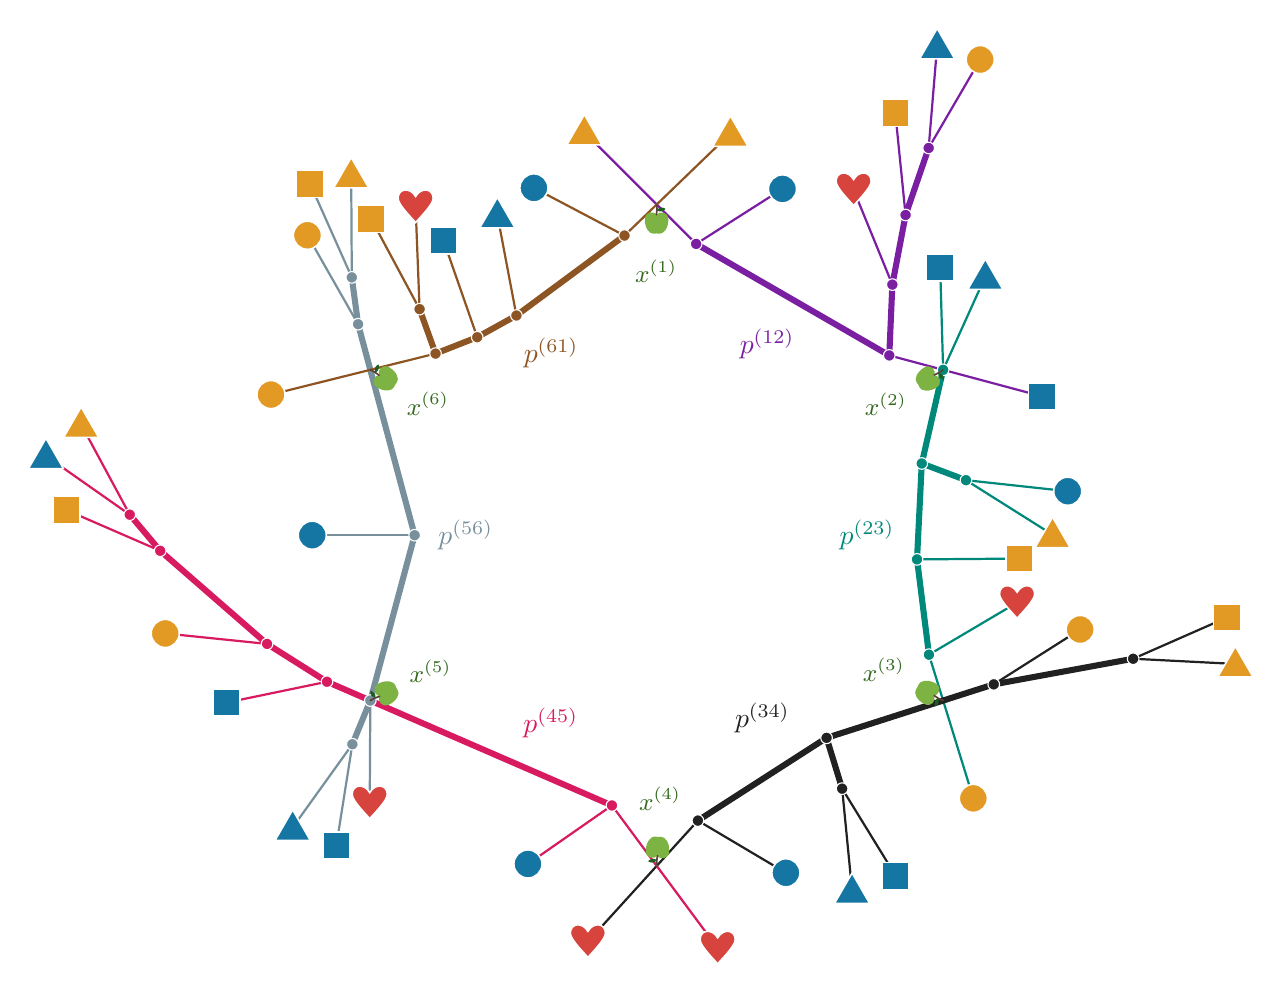
\begin{tikzpicture}[x=1cm,y=1cm]
% p^(12)
\draw[hex pendant,draw=hexTree1] (1.5971,4.3978)--(0.5007,3.6993);
\draw[hex pendant,draw=hexTree1] (3.5612,6.2131)--(3.4535,4.9176);
\draw[hex pendant,draw=hexTree1] (4.8930,1.7635)--(3.6373,2.1000);
\draw[hex pendant,draw=hexTree1] (3.0303,5.3601)--(3.1605,4.0666);
\draw[hex pendant,draw=hexTree1] (-0.9192,5.1192)--(0.0000,4.2000);
\draw[hex pendant,draw=hexTree1] (4.1084,6.0406)--(3.4535,4.9176);
\draw[hex internal,draw=hexTree1] (0.5007,3.6993)--(2.9534,2.2833);
\draw[hex pendant,draw=hexTree1] (0.5007,3.6993)--(0.0000,4.2000);
\draw[hex pendant,draw=hexTree1] (2.5004,4.3856)--(2.9926,3.1824);
\draw[hex internal,draw=hexTree1] (3.4535,4.9176)--(3.1605,4.0666);
\draw[hex internal,draw=hexTree1] (3.1605,4.0666)--(2.9926,3.1824);
\draw[hex internal,draw=hexTree1] (2.9534,2.2833)--(2.9926,3.1824);
\draw[hex pendant,draw=hexTree1] (2.9534,2.2833)--(3.6373,2.1000);
\node[hex vertex,fill=hexTree1] at (0.5007,3.6993) {};
\node[hex vertex,fill=hexTree1] at (3.4535,4.9176) {};
\node[hex vertex,fill=hexTree1] at (3.1605,4.0666) {};
\node[hex vertex,fill=hexTree1] at (2.9926,3.1824) {};
\node[hex vertex,fill=hexTree1] at (2.9534,2.2833) {};
\coordinate (v1) at (4.8930,1.7635);
\node[g2tree dark,rectangle,minimum size=3.4155000000000006mm,font={\sffamily\fontsize{6.6}{6.6}\selectfont\bfseries}] at (v1) {};
\coordinate (v2) at (3.5612,6.2131);
\begin{scope}[shift={(v2)},scale=0.7425000000000002,transform shape]
\path[fill=g2TaxonBlue,draw=white,line width=.55pt,line join=round] (0mm,3.0mm)--(-3.0mm,-2.2mm)--(3.0mm,-2.2mm)--cycle;
\end{scope}
\coordinate (v3) at (1.5971,4.3978);
\node[g2tree dark,circle,minimum size=3.5640000000000005mm,font={\sffamily\fontsize{6.6}{6.6}\selectfont\bfseries}] at (v3) {};
\coordinate (v4) at (3.0303,5.3601);
\node[g2tree light,rectangle,minimum size=3.4155000000000006mm,font={\sffamily\fontsize{6.6}{6.6}\selectfont\bfseries}] at (v4) {};
\coordinate (v5) at (-0.9192,5.1192);
\begin{scope}[shift={(v5)},scale=0.7425000000000002,transform shape]
\path[fill=g2TaxonYellow,draw=white,line width=.55pt,line join=round] (0mm,3.0mm)--(-3.0mm,-2.2mm)--(3.0mm,-2.2mm)--cycle;
\end{scope}
\coordinate (v6) at (4.1084,6.0406);
\node[g2tree light,circle,minimum size=3.5640000000000005mm,font={\sffamily\fontsize{6.6}{6.6}\selectfont\bfseries}] at (v6) {};
\coordinate (v7) at (2.5004,4.3856);
\begin{scope}[shift={(v7)},scale=0.7425000000000002,transform shape]
\path[fill=g2HeartRed,draw=white,line width=.55pt]
  (0mm,-2.7mm)..controls(-.45mm,-2.1mm)and(-3.0mm,.35mm)..(-3.0mm,1.45mm)
  ..controls(-3.0mm,3.2mm)and(-.9mm,3.4mm)..(0mm,1.75mm)
  ..controls(.9mm,3.4mm)and(3.0mm,3.2mm)..(3.0mm,1.45mm)
  ..controls(3.0mm,.35mm)and(.45mm,-2.1mm)..(0mm,-2.7mm)--cycle;
\end{scope}
% p^(23)
\draw[hex pendant,draw=hexTree2] (5.2198,0.5583)--(3.9274,0.6988);
\draw[hex pendant,draw=hexTree2] (4.1732,3.2844)--(3.6373,2.1000);
\draw[hex pendant,draw=hexTree2] (3.5998,3.3995)--(3.6373,2.1000);
\draw[hex pendant,draw=hexTree2] (4.6055,-0.2972)--(3.3056,-0.3072);
\draw[hex pendant,draw=hexTree2] (5.0274,0.0060)--(3.9274,0.6988);
\draw[hex pendant,draw=hexTree2] (4.0207,-3.3422)--(3.6373,-2.1000);
\draw[hex internal,draw=hexTree2] (3.4575,-1.5173)--(3.3056,-0.3072);
\draw[hex pendant,draw=hexTree2] (3.4575,-1.5173)--(3.6373,-2.1000);
\draw[hex pendant,draw=hexTree2] (4.5766,-0.8559)--(3.4575,-1.5173);
\draw[hex internal,draw=hexTree2] (3.9274,0.6988)--(3.3661,0.9109);
\draw[hex internal,draw=hexTree2] (3.3056,-0.3072)--(3.3661,0.9109);
\draw[hex internal,draw=hexTree2] (3.6373,2.1000)--(3.3661,0.9109);
\node[hex vertex,fill=hexTree2] at (3.4575,-1.5173) {};
\node[hex vertex,fill=hexTree2] at (3.9274,0.6988) {};
\node[hex vertex,fill=hexTree2] at (3.3056,-0.3072) {};
\node[hex vertex,fill=hexTree2] at (3.3661,0.9109) {};
\node[hex vertex,fill=hexTree2] at (3.6373,2.1000) {};
\coordinate (v1) at (3.5998,3.3995);
\node[g2tree dark,rectangle,minimum size=3.4155000000000006mm,font={\sffamily\fontsize{6.6}{6.6}\selectfont\bfseries}] at (v1) {};
\coordinate (v2) at (4.1732,3.2844);
\begin{scope}[shift={(v2)},scale=0.7425000000000002,transform shape]
\path[fill=g2TaxonBlue,draw=white,line width=.55pt,line join=round] (0mm,3.0mm)--(-3.0mm,-2.2mm)--(3.0mm,-2.2mm)--cycle;
\end{scope}
\coordinate (v3) at (5.2198,0.5583);
\node[g2tree dark,circle,minimum size=3.5640000000000005mm,font={\sffamily\fontsize{6.6}{6.6}\selectfont\bfseries}] at (v3) {};
\coordinate (v4) at (4.6055,-0.2972);
\node[g2tree light,rectangle,minimum size=3.4155000000000006mm,font={\sffamily\fontsize{6.6}{6.6}\selectfont\bfseries}] at (v4) {};
\coordinate (v5) at (5.0274,0.0060);
\begin{scope}[shift={(v5)},scale=0.7425000000000002,transform shape]
\path[fill=g2TaxonYellow,draw=white,line width=.55pt,line join=round] (0mm,3.0mm)--(-3.0mm,-2.2mm)--(3.0mm,-2.2mm)--cycle;
\end{scope}
\coordinate (v6) at (4.0207,-3.3422);
\node[g2tree light,circle,minimum size=3.5640000000000005mm,font={\sffamily\fontsize{6.6}{6.6}\selectfont\bfseries}] at (v6) {};
\coordinate (v7) at (4.5766,-0.8559);
\begin{scope}[shift={(v7)},scale=0.7425000000000002,transform shape]
\path[fill=g2HeartRed,draw=white,line width=.55pt]
  (0mm,-2.7mm)..controls(-.45mm,-2.1mm)and(-3.0mm,.35mm)..(-3.0mm,1.45mm)
  ..controls(-3.0mm,3.2mm)and(-.9mm,3.4mm)..(0mm,1.75mm)
  ..controls(.9mm,3.4mm)and(3.0mm,3.2mm)..(3.0mm,1.45mm)
  ..controls(3.0mm,.35mm)and(.45mm,-2.1mm)..(0mm,-2.7mm)--cycle;
\end{scope}
% p^(34)
\draw[hex pendant,draw=hexTree3] (1.6408,-4.2877)--(0.5226,-3.6247);
\draw[hex pendant,draw=hexTree3] (2.4809,-4.5129)--(2.3549,-3.2190);
\draw[hex pendant,draw=hexTree3] (3.0354,-4.3267)--(2.3549,-3.2190);
\draw[hex pendant,draw=hexTree3] (7.2405,-1.0455)--(6.0506,-1.5690);
\draw[hex pendant,draw=hexTree3] (7.3489,-1.6352)--(6.0506,-1.5690);
\draw[hex pendant,draw=hexTree3] (5.3777,-1.1975)--(4.2802,-1.8943);
\draw[hex internal,draw=hexTree3] (6.0506,-1.5690)--(4.2802,-1.8943);
\draw[hex pendant,draw=hexTree3] (-0.8742,-5.1622)--(0.0000,-4.2000);
\draw[hex internal,draw=hexTree3] (0.5226,-3.6247)--(2.1569,-2.5738);
\draw[hex pendant,draw=hexTree3] (0.5226,-3.6247)--(0.0000,-4.2000);
\draw[hex internal,draw=hexTree3] (2.1569,-2.5738)--(3.6373,-2.1000);
\draw[hex internal,draw=hexTree3] (2.3549,-3.2190)--(2.1569,-2.5738);
\draw[hex internal,draw=hexTree3] (4.2802,-1.8943)--(3.6373,-2.1000);
\node[hex vertex,fill=hexTree3] at (6.0506,-1.5690) {};
\node[hex vertex,fill=hexTree3] at (0.5226,-3.6247) {};
\node[hex vertex,fill=hexTree3] at (2.3549,-3.2190) {};
\node[hex vertex,fill=hexTree3] at (2.1569,-2.5738) {};
\node[hex vertex,fill=hexTree3] at (4.2802,-1.8943) {};
\coordinate (v1) at (3.0354,-4.3267);
\node[g2tree dark,rectangle,minimum size=3.4155000000000006mm,font={\sffamily\fontsize{6.6}{6.6}\selectfont\bfseries}] at (v1) {};
\coordinate (v2) at (2.4809,-4.5129);
\begin{scope}[shift={(v2)},scale=0.7425000000000002,transform shape]
\path[fill=g2TaxonBlue,draw=white,line width=.55pt,line join=round] (0mm,3.0mm)--(-3.0mm,-2.2mm)--(3.0mm,-2.2mm)--cycle;
\end{scope}
\coordinate (v3) at (1.6408,-4.2877);
\node[g2tree dark,circle,minimum size=3.5640000000000005mm,font={\sffamily\fontsize{6.6}{6.6}\selectfont\bfseries}] at (v3) {};
\coordinate (v4) at (7.2405,-1.0455);
\node[g2tree light,rectangle,minimum size=3.4155000000000006mm,font={\sffamily\fontsize{6.6}{6.6}\selectfont\bfseries}] at (v4) {};
\coordinate (v5) at (7.3489,-1.6352);
\begin{scope}[shift={(v5)},scale=0.7425000000000002,transform shape]
\path[fill=g2TaxonYellow,draw=white,line width=.55pt,line join=round] (0mm,3.0mm)--(-3.0mm,-2.2mm)--(3.0mm,-2.2mm)--cycle;
\end{scope}
\coordinate (v6) at (5.3777,-1.1975);
\node[g2tree light,circle,minimum size=3.5640000000000005mm,font={\sffamily\fontsize{6.6}{6.6}\selectfont\bfseries}] at (v6) {};
\coordinate (v7) at (-0.8742,-5.1622);
\begin{scope}[shift={(v7)},scale=0.7425000000000002,transform shape]
\path[fill=g2HeartRed,draw=white,line width=.55pt]
  (0mm,-2.7mm)..controls(-.45mm,-2.1mm)and(-3.0mm,.35mm)..(-3.0mm,1.45mm)
  ..controls(-3.0mm,3.2mm)and(-.9mm,3.4mm)..(0mm,1.75mm)
  ..controls(.9mm,3.4mm)and(3.0mm,3.2mm)..(3.0mm,1.45mm)
  ..controls(3.0mm,.35mm)and(.45mm,-2.1mm)..(0mm,-2.7mm)--cycle;
\end{scope}
% p^(45)
\draw[hex pendant,draw=hexTree4] (-1.6356,-4.1752)--(-0.5689,-3.4321);
\draw[hex pendant,draw=hexTree4] (-7.7566,1.0075)--(-6.6925,0.2606);
\draw[hex pendant,draw=hexTree4] (-5.4605,-2.1254)--(-4.1877,-1.8611);
\draw[hex pendant,draw=hexTree4] (-7.4983,0.3196)--(-6.3058,-0.1981);
\draw[hex pendant,draw=hexTree4] (-7.3095,1.4049)--(-6.6925,0.2606);
\draw[hex pendant,draw=hexTree4] (-6.2419,-1.2477)--(-4.9487,-1.3806);
\draw[hex pendant,draw=hexTree4] (-0.5689,-3.4321)--(0.0000,-4.2000);
\draw[hex internal,draw=hexTree4] (-0.5689,-3.4321)--(-3.6373,-2.1000);
\draw[hex pendant,draw=hexTree4] (0.7739,-5.2446)--(0.0000,-4.2000);
\draw[hex internal,draw=hexTree4] (-4.9487,-1.3806)--(-6.3058,-0.1981);
\draw[hex internal,draw=hexTree4] (-6.6925,0.2606)--(-6.3058,-0.1981);
\draw[hex internal,draw=hexTree4] (-4.1877,-1.8611)--(-4.9487,-1.3806);
\draw[hex internal,draw=hexTree4] (-4.1877,-1.8611)--(-3.6373,-2.1000);
\node[hex vertex,fill=hexTree4] at (-0.5689,-3.4321) {};
\node[hex vertex,fill=hexTree4] at (-4.9487,-1.3806) {};
\node[hex vertex,fill=hexTree4] at (-6.6925,0.2606) {};
\node[hex vertex,fill=hexTree4] at (-6.3058,-0.1981) {};
\node[hex vertex,fill=hexTree4] at (-4.1877,-1.8611) {};
\coordinate (v1) at (-5.4605,-2.1254);
\node[g2tree dark,rectangle,minimum size=3.4155000000000006mm,font={\sffamily\fontsize{6.6}{6.6}\selectfont\bfseries}] at (v1) {};
\coordinate (v2) at (-7.7566,1.0075);
\begin{scope}[shift={(v2)},scale=0.7425000000000002,transform shape]
\path[fill=g2TaxonBlue,draw=white,line width=.55pt,line join=round] (0mm,3.0mm)--(-3.0mm,-2.2mm)--(3.0mm,-2.2mm)--cycle;
\end{scope}
\coordinate (v3) at (-1.6356,-4.1752);
\node[g2tree dark,circle,minimum size=3.5640000000000005mm,font={\sffamily\fontsize{6.6}{6.6}\selectfont\bfseries}] at (v3) {};
\coordinate (v4) at (-7.4983,0.3196);
\node[g2tree light,rectangle,minimum size=3.4155000000000006mm,font={\sffamily\fontsize{6.6}{6.6}\selectfont\bfseries}] at (v4) {};
\coordinate (v5) at (-7.3095,1.4049);
\begin{scope}[shift={(v5)},scale=0.7425000000000002,transform shape]
\path[fill=g2TaxonYellow,draw=white,line width=.55pt,line join=round] (0mm,3.0mm)--(-3.0mm,-2.2mm)--(3.0mm,-2.2mm)--cycle;
\end{scope}
\coordinate (v6) at (-6.2419,-1.2477);
\node[g2tree light,circle,minimum size=3.5640000000000005mm,font={\sffamily\fontsize{6.6}{6.6}\selectfont\bfseries}] at (v6) {};
\coordinate (v7) at (0.7739,-5.2446);
\begin{scope}[shift={(v7)},scale=0.7425000000000002,transform shape]
\path[fill=g2HeartRed,draw=white,line width=.55pt]
  (0mm,-2.7mm)..controls(-.45mm,-2.1mm)and(-3.0mm,.35mm)..(-3.0mm,1.45mm)
  ..controls(-3.0mm,3.2mm)and(-.9mm,3.4mm)..(0mm,1.75mm)
  ..controls(.9mm,3.4mm)and(3.0mm,3.2mm)..(3.0mm,1.45mm)
  ..controls(3.0mm,.35mm)and(.45mm,-2.1mm)..(0mm,-2.7mm)--cycle;
\end{scope}
% p^(56)
\draw[hex pendant,draw=hexTree5] (-4.3746,0.0000)--(-3.0746,0.0000);
\draw[hex pendant,draw=hexTree5] (-4.6233,-3.7111)--(-3.8653,-2.6550);
\draw[hex pendant,draw=hexTree5] (-4.0687,-3.9390)--(-3.8653,-2.6550);
\draw[hex pendant,draw=hexTree5] (-4.4014,4.4618)--(-3.8726,3.2742);
\draw[hex pendant,draw=hexTree5] (-3.8802,4.5742)--(-3.8726,3.2742);
\draw[hex pendant,draw=hexTree5] (-4.4360,3.8092)--(-3.7926,2.6796);
\draw[hex internal,draw=hexTree5] (-3.8726,3.2742)--(-3.7926,2.6796);
\draw[hex pendant,draw=hexTree5] (-3.6449,-3.4000)--(-3.6373,-2.1000);
\draw[hex internal,draw=hexTree5] (-3.0746,0.0000)--(-3.6373,-2.1000);
\draw[hex internal,draw=hexTree5] (-3.0746,0.0000)--(-3.6373,2.1000);
\draw[hex internal,draw=hexTree5] (-3.8653,-2.6550)--(-3.6373,-2.1000);
\draw[hex internal,draw=hexTree5] (-3.7926,2.6796)--(-3.6373,2.1000);
\node[hex vertex,fill=hexTree5] at (-3.8726,3.2742) {};
\node[hex vertex,fill=hexTree5] at (-3.0746,0.0000) {};
\node[hex vertex,fill=hexTree5] at (-3.8653,-2.6550) {};
\node[hex vertex,fill=hexTree5] at (-3.6373,-2.1000) {};
\node[hex vertex,fill=hexTree5] at (-3.7926,2.6796) {};
\coordinate (v1) at (-4.0687,-3.9390);
\node[g2tree dark,rectangle,minimum size=3.4155000000000006mm,font={\sffamily\fontsize{6.6}{6.6}\selectfont\bfseries}] at (v1) {};
\coordinate (v2) at (-4.6233,-3.7111);
\begin{scope}[shift={(v2)},scale=0.7425000000000002,transform shape]
\path[fill=g2TaxonBlue,draw=white,line width=.55pt,line join=round] (0mm,3.0mm)--(-3.0mm,-2.2mm)--(3.0mm,-2.2mm)--cycle;
\end{scope}
\coordinate (v3) at (-4.3746,0.0000);
\node[g2tree dark,circle,minimum size=3.5640000000000005mm,font={\sffamily\fontsize{6.6}{6.6}\selectfont\bfseries}] at (v3) {};
\coordinate (v4) at (-4.4014,4.4618);
\node[g2tree light,rectangle,minimum size=3.4155000000000006mm,font={\sffamily\fontsize{6.6}{6.6}\selectfont\bfseries}] at (v4) {};
\coordinate (v5) at (-3.8802,4.5742);
\begin{scope}[shift={(v5)},scale=0.7425000000000002,transform shape]
\path[fill=g2TaxonYellow,draw=white,line width=.55pt,line join=round] (0mm,3.0mm)--(-3.0mm,-2.2mm)--(3.0mm,-2.2mm)--cycle;
\end{scope}
\coordinate (v6) at (-4.4360,3.8092);
\node[g2tree light,circle,minimum size=3.5640000000000005mm,font={\sffamily\fontsize{6.6}{6.6}\selectfont\bfseries}] at (v6) {};
\coordinate (v7) at (-3.6449,-3.4000);
\begin{scope}[shift={(v7)},scale=0.7425000000000002,transform shape]
\path[fill=g2HeartRed,draw=white,line width=.55pt]
  (0mm,-2.7mm)..controls(-.45mm,-2.1mm)and(-3.0mm,.35mm)..(-3.0mm,1.45mm)
  ..controls(-3.0mm,3.2mm)and(-.9mm,3.4mm)..(0mm,1.75mm)
  ..controls(.9mm,3.4mm)and(3.0mm,3.2mm)..(3.0mm,1.45mm)
  ..controls(3.0mm,.35mm)and(.45mm,-2.1mm)..(0mm,-2.7mm)--cycle;
\end{scope}
% p^(61)
\draw[hex pendant,draw=hexTree6] (-1.5597,4.4107)--(-0.4094,3.8049);
\draw[hex pendant,draw=hexTree6] (-2.0239,4.0674)--(-1.7819,2.7901);
\draw[hex pendant,draw=hexTree6] (-2.7078,3.7420)--(-2.2797,2.5145);
\draw[hex pendant,draw=hexTree6] (-3.6265,4.0163)--(-3.0117,2.8709);
\draw[hex pendant,draw=hexTree6] (0.9355,5.1027)--(0.0000,4.2000);
\draw[hex pendant,draw=hexTree6] (-4.8988,1.7860)--(-3.6373,2.1000);
\draw[hex internal,draw=hexTree6] (-0.4094,3.8049)--(-1.7819,2.7901);
\draw[hex pendant,draw=hexTree6] (-0.4094,3.8049)--(0.0000,4.2000);
\draw[hex pendant,draw=hexTree6] (-3.0622,4.1700)--(-3.0117,2.8709);
\draw[hex internal,draw=hexTree6] (-2.2797,2.5145)--(-2.8091,2.3062);
\draw[hex pendant,draw=hexTree6] (-2.8091,2.3062)--(-3.6373,2.1000);
\draw[hex internal,draw=hexTree6] (-3.0117,2.8709)--(-2.8091,2.3062);
\draw[hex internal,draw=hexTree6] (-1.7819,2.7901)--(-2.2797,2.5145);
\node[hex vertex,fill=hexTree6] at (-0.4094,3.8049) {};
\node[hex vertex,fill=hexTree6] at (-2.2797,2.5145) {};
\node[hex vertex,fill=hexTree6] at (-3.0117,2.8709) {};
\node[hex vertex,fill=hexTree6] at (-2.8091,2.3062) {};
\node[hex vertex,fill=hexTree6] at (-1.7819,2.7901) {};
\coordinate (v1) at (-2.7078,3.7420);
\node[g2tree dark,rectangle,minimum size=3.4155000000000006mm,font={\sffamily\fontsize{6.6}{6.6}\selectfont\bfseries}] at (v1) {};
\coordinate (v2) at (-2.0239,4.0674);
\begin{scope}[shift={(v2)},scale=0.7425000000000002,transform shape]
\path[fill=g2TaxonBlue,draw=white,line width=.55pt,line join=round] (0mm,3.0mm)--(-3.0mm,-2.2mm)--(3.0mm,-2.2mm)--cycle;
\end{scope}
\coordinate (v3) at (-1.5597,4.4107);
\node[g2tree dark,circle,minimum size=3.5640000000000005mm,font={\sffamily\fontsize{6.6}{6.6}\selectfont\bfseries}] at (v3) {};
\coordinate (v4) at (-3.6265,4.0163);
\node[g2tree light,rectangle,minimum size=3.4155000000000006mm,font={\sffamily\fontsize{6.6}{6.6}\selectfont\bfseries}] at (v4) {};
\coordinate (v5) at (0.9355,5.1027);
\begin{scope}[shift={(v5)},scale=0.7425000000000002,transform shape]
\path[fill=g2TaxonYellow,draw=white,line width=.55pt,line join=round] (0mm,3.0mm)--(-3.0mm,-2.2mm)--(3.0mm,-2.2mm)--cycle;
\end{scope}
\coordinate (v6) at (-4.8988,1.7860);
\node[g2tree light,circle,minimum size=3.5640000000000005mm,font={\sffamily\fontsize{6.6}{6.6}\selectfont\bfseries}] at (v6) {};
\coordinate (v7) at (-3.0622,4.1700);
\begin{scope}[shift={(v7)},scale=0.7425000000000002,transform shape]
\path[fill=g2HeartRed,draw=white,line width=.55pt]
  (0mm,-2.7mm)..controls(-.45mm,-2.1mm)and(-3.0mm,.35mm)..(-3.0mm,1.45mm)
  ..controls(-3.0mm,3.2mm)and(-.9mm,3.4mm)..(0mm,1.75mm)
  ..controls(.9mm,3.4mm)and(3.0mm,3.2mm)..(3.0mm,1.45mm)
  ..controls(3.0mm,.35mm)and(.45mm,-2.1mm)..(0mm,-2.7mm)--cycle;
\end{scope}
\pic[rotate=-0.5,scale=0.650] at (0.0000,4.2000) {g2apple};
\node[hex point label] at (-0.0076,3.3500) {\(x^{(1)}\)};
\node[hex line label,text=hexTree1] at (1.4020,2.4284) {\(p^{(12)}\)};
\pic[rotate=-58.9,scale=0.650] at (3.6373,2.1000) {g2apple};
\node[hex point label] at (2.9093,1.6612) {\(x^{(2)}\)};
\node[hex line label,text=hexTree2] at (2.6707,-0.0021) {\(p^{(23)}\)};
\pic[rotate=242.4,scale=0.650] at (3.6373,-2.1000) {g2apple};
\node[hex point label] at (2.8837,-1.7068) {\(x^{(3)}\)};
\node[hex line label,text=hexTree3] at (1.3418,-2.3260) {\(p^{(34)}\)};
\pic[rotate=177.1,scale=0.650] at (0.0000,-4.2000) {g2apple};
\node[hex point label] at (0.0424,-3.3511) {\(x^{(4)}\)};
\node[hex line label,text=hexTree4] at (-1.3458,-2.3900) {\(p^{(45)}\)};
\pic[rotate=115.8,scale=0.650] at (-3.6373,-2.1000) {g2apple};
\node[hex point label] at (-2.8718,-1.7305) {\(x^{(5)}\)};
\node[hex line label,text=hexTree5] at (-2.4246,0.0000) {\(p^{(56)}\)};
\pic[rotate=59.5,scale=0.650] at (-3.6373,2.1000) {g2apple};
\node[hex point label] at (-2.9050,1.6685) {\(x^{(6)}\)};
\node[hex line label,text=hexTree6] at (-1.3414,2.3124) {\(p^{(61)}\)};
\end{tikzpicture}
\endgroup
